\documentclass{fizykalab}

% Variables
\def\pomvspace{\vspace{0.3em}}

% Ustawienia strony
\usepackage{lipsum}
\usepackage[margin=3cm]{geometry}
\usepackage{graphicx}
\usepackage{enumitem}
\usepackage{siunitx}
\usepackage{amsmath}
\usepackage{cancel}
\usepackage{makecell}
\usepackage{mathtools}
\setlist{leftmargin=15pt,labelindent=15pt}
\setlist[enumerate]{noitemsep,wide=0pt, leftmargin=*}

% Ustawienia stopki
\usepackage{lastpage}
\usepackage{fancyhdr}
\pagestyle{fancy}
\fancyhf{} % sets both header and footer to nothing
\renewcommand{\headrulewidth}{0pt}
\cfoot{\thepage\ z \pageref{LastPage}}

% Ustawienia do tabelki
\wydzial{IEiT}
\autorjeden{Robert Mesek}
\autordwa{}
\rok{II}
\grupa{8 - L}
\zespol{6}
\temat{Elektroliza}
\nrcwiczenia{35}
\datawykonania{7.11.2023}
\dataoddaniajeden{}
\zwrotdopoprawy{}
\dataoddaniadwa{}
\datazaliczenia{}

\begin{document}

\maketitle
{\setlength{\parindent}{0pt}
\section*{Ćwiczenie "35": Elektroliza}
\subsection*{Cel ćwiczenia}
\par
Pomiar różnicy mas miedzianych elektrod po przeprowadzeniu elektrolizy, w celu 
wyznaczenia wartości równoważnika elektrochemicznego $k$ miedzi, stałej Faradaya $F$ oraz ładunku elementarnego $e$.

\subsection*{Opis ćwiczenia}
\par
Liczba atomów wydzielonych na elektrodzie jest stosunkiem ładunku całkowitego
(czyli iloczynu prądu $I$ i czasu $t$) do ładunku pojedynczego jonu:
\begin{gather*}
	N = \frac{It}{we} \ .
	\tag{1}
\end{gather*}

Masę powstałych atomów można obliczyć mnożąc liczbę atomów $N$ przez masę
pojedynczego atomu równą stosunkowi masy molowej $\mu$ do liczby Avogadra $N_A$, czyli:
\begin{gather*}
	m = N \frac{\mu}{N_A} = \frac{\mu}{weN_A}It \ .
	\tag{2}
\end{gather*}

Elektrochemicznym równoważnikiem substancji:
\begin{gather*}
	k = \frac{\mu}{weN_A}
	\tag{3}
\end{gather*}

Wzór użyty do obliczenia $k$ z (2) i (3):
\begin{gather*}
	m = kIt \ \Rightarrow \ k = \frac{m}{It}
	\tag{4}
\end{gather*}

Wzór użyty do obliczenia stałej Faradaya $F = eN_A$:
\begin{gather*}
	k = \frac{\mu}{weN_A} = \frac{\mu}{wF} \\
	\Downarrow \\
	F = \frac{\mu}{wk}
	\tag{5}
\end{gather*}

Wzór użyty do obliczenia wartości ładunku elementarnego po przekształceniu $F = eN_A$:
\begin{gather*}
	e = \frac{F}{N_A}
	\tag{6}
\end{gather*}
\newpage

\section*{Stanowisko pomiarowe}
\par
Układ pomiarowy (Rys. 1) składa się z:

\quad 1. Naczynie do elektrolizy siarczanu miedzi CuSO\textsubscript{4} z miedzianymi elektrodami 

\quad \ \ w kształcie równoległych płyt, oddalonych od siebie o kilka centymetrów (rys. 1). 

\quad 2. Zasilacz napięcia stałego

\quad 3. Amperomierz

\quad 4. Opornica suwakowa

\quad 5. Waga elektroniczna

\begin{figure}[!ht]
	\centering
	\vspace{0pt}
	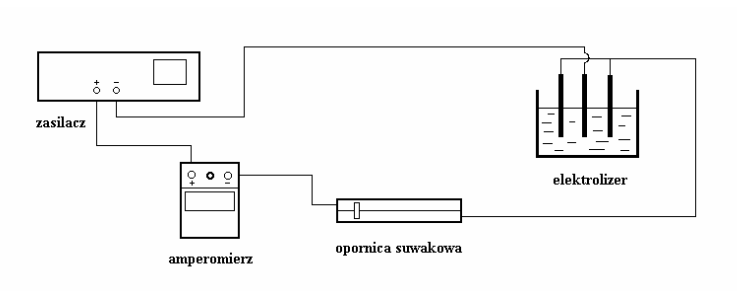
\includegraphics[width=0.9\linewidth]{images/uklad1.png}
	\caption*{Rys. 1 Układ pomiarowy}
\end{figure}



\section*{Przebieg doświadczenia}
\par
Przed rozpoczęciem doświadczenia elektrody zostały dokładnie wyczyszczone przy pomocy papieru ściernego oraz wody destylowanej. 

Następnie wszystkie trzy elektrody zważono, włożono do układu, ustawiono odpowiednie napięcie prądu oraz opór, by uzyskać wartość natężenia prądu $I = 0.5 A$. 
W trakcie trwania elektrolizy, kontrolowano czy płytki były dobrze zanurzone w roztworze oraz obwód działa prawidłowo. 

Po odczekaniu 30 minut elektrody wyjęto z elektrolitu i po wysuszeniu ich suszarką ponownie zważono.

\newpage

\section*{Wyniki pomiarów}
\par
\begin{table}[H]
	\centering
	\begin{tabular}{|l|l|}
		\hline
		\rule{0pt}{1em} Czas elektrolizy $t$ & 30 min. \\ \hline
		\rule{0pt}{1em} Natężenie prądu $I$ & 0.5 $A$ \\ \hline\hline
		\rule{0pt}{1em} Masa katody przed elektrolizą $m_{K1}$ & 81.977 $g$ \\ \hline
		\rule{0pt}{1em} Masa katody po elektrolizą $m_{K2}$ & 82.265 $g$ \\ \hline
		\rule{0pt}{1em} Różnica masy katody $\Delta m_K$ & 0.288 $g$ \\ \hline\hline
		\rule{0pt}{1em} Masa anod przed elektrolizą $M_{A1}$ & 175.409 $g$ \\ \hline
		\rule{0pt}{1em} Masa anod po elektrolizą $M_{A2}$ & 175.116 $g$ \\ \hline
		\rule{0pt}{1em} Różnica masy anod $\Delta M_A$ & 0.293 $g$ \\ \hline
	\end{tabular}
	\caption*{Tabela 1: Pomiary parametrów elektrolizy.}
\end{table}

\section*{Dane określające niepewność przyrządów}
\par
\begin{table}[H]
	\centering
	\begin{tabular}{|l|l|}
		\hline
		\rule{0pt}{1em} Klasa amperomierza & $0.5$ \\ \hline
		\rule{0pt}{1em} Używany zakres amperomierza & $750 \ mA$ \\ \hline
		\rule{0pt}{1em} Niepewność amperomierza & $\Delta I = \frac{0.5 \cdot 0.75 A}{100} \approx 0.004 \ A$ \\ \hline
		\rule{0pt}{1em} Niepewność graniczna wagi (znamionowa) & $ \Delta m = 0.001 \ g$ \\ \hline
	\end{tabular}
	\caption*{Tabela 2: Niepewności przyrządów.}
\end{table}

\section*{Opracowanie wyników}
\subsection*{Niepewności pomiarowe}
\par
Niepewność pomiaru czasu spowodowane czasem reakcji człowieka oraz opóźnieniem uruchamiania i wyłączania przyrządów:
\begin{gather*}
	u(t) = 2 \ s 
\end{gather*}

Niepewność standardowa wagi powiększona o różnicę mas wynikającą z mycia oraz suszenia płytek ($5 \ mg$):
\begin{gather*}
	u(m) = \frac{\Delta m}{\sqrt{3}} + 0.005 \ g \approx 0.0056 \ g
\end{gather*}

Niepewność standardowa amperomierza:
\begin{gather*}
	u(I) = \frac{\Delta I}{\sqrt{3}} \approx 0.0023 \ A
\end{gather*}


\newpage

\subsection*{Wyznaczenie równoważnika elektrochemicznego miedzi}
\par
Do obliczenia równoważnika elektrochemicznego miedzi $k$ skorzystamy z wyprowadzonego wzoru (4):
\begin{gather*}
	k = \frac{m}{It}
\end{gather*}
gdzie masa wydzielonej substancji to zmiana masy katody $\Delta m_K$:
\begin{gather*}
	k = \frac{0.288g}{0.5A \cdot 1800s} = 0.00032 \ \frac{g}{A \cdot s} = 0.320 \ \frac{mg}{A \cdot s}
\end{gather*}
Niepewność pomiarowa równoważnika elektrochemicznego obliczona z prawa przenoszenia niepewności:
\begin{gather*}
	u(k) = \sqrt{\left(\frac{\partial k}{\partial m}u(m)\right)^2 + \left(\frac{\partial k}{\partial I}u(I)\right)^2 + \left(\frac{\partial k}{\partial t}u(t)\right)^2} = \\
	= \sqrt{\left(\frac{1}{It}u(m)\right)^2 + \left(-\frac{m}{I^2t}u(I)\right)^2 + \left(-\frac{m}{It^2}u(t)\right)^2} \approx \\
	\approx 6.4 \cdot 10^{-6} \ \frac{g}{A \cdot s} = 0.0064 \ \frac{mg}{A \cdot s} \\
	\frac{u(k)}{k} = 2 \%
\end{gather*}

\subsection*{Wyznaczenie stałej Faradaya}
\par
Do obliczenia stałej Faradaya wykorzystamy wzór (5), podstawiając wartości tablicowe dla miedzi $w = 2$, $\mu = 63.55 \ g$ oraz otrzymaną wartość $k$:
\begin{gather*}
	F = \frac{\mu}{wk} \approx 99297 \ \frac{C}{mol}
\end{gather*}
Niepewność pomiarowa obliczona z prawa przenoszenia niepewności:
\begin{gather*}
	u(F) = \sqrt{\left(\frac{\partial F}{\partial k} u(k)\right)^2} = \left|\frac{\mu}{wk^2} u(k)\right| \approx 1986 \ \frac{C}{mol} \\
	\frac{u(F)}{F} \approx 2 \%
\end{gather*}

\subsection*{Wyznaczanie wartości ładunku elementarnego}
\par
Wartość ładunku elementarnego wyznaczymy ze wzoru (6) przyjmując stała Avogadra \\ $N_A = 6.0221 \cdot 10^{23} \frac{1}{mol}$.
\begin{gather*}
	e = \frac{F}{N_A} \approx 1.65 \cdot 10^{-19} \ C
\end{gather*}

Niepewność pomiarowa obliczona z prawa przenoszenia niepewności:
\begin{gather*}
	u(e) = \sqrt{\left(\frac{\partial e}{\partial F} u(F)\right)^2} = \left|\frac{1}{N_A} u(F)\right| \approx 3.3 \cdot 10^{-21} \ C \\
	\frac{u(e)}{e} \approx 2 \%
\end{gather*}

\newpage

\subsection*{Porównanie z wartościami tabelarycznymi}
\begin{table}[H]
	\centering
	\begin{tabular}{|l|l|l|l|}
		\hline
		\rule{0pt}{1em} \textbf{Stała} & \textbf{Obliczona wartość} & \textbf{Tabelaryczna wartość} & \textbf{Różnica} \\ \hline\hline
		\rule{0pt}{1em} \makecell{Równoważnik \\ elektrochemiczny $k$} & $0.320 \pm 0.006 \ \frac{mg}{A \cdot s}$ & $0.329 \ \frac{mg}{A \cdot s}$ & $0.009 \ \frac{mg}{A \cdot s}$ \\ \hline
		\rule{0pt}{1em} Stała Faradaya $F$ & $99297 \pm 1986 \ \frac{C}{mol}$ & $96485 \ \frac{C}{mol}$ & $2812 \ \frac{C}{mol}$ \\ \hline
		\rule{0pt}{1em} Ładunek elementarny $e$ & $(1.65 \pm 0.03) \cdot 10^{-19} \ C$ & $1.60 \cdot 10^{-19} \ C$ & $0.05 \cdot 10^{-19} \ C$ \\ \hline
	\end{tabular}
	\caption*{Tabela 3: Różnica pomiędzy otrzymanymi a tabelarycznymi wartościami}
\end{table}

\section*{Wnioski}
\par
Otrzymane wyniki są zgodne z przewidywanymi oraz błędy względne równe około 2\% są akceptowalne.

Z dość dużą dokładnością udało wyznaczyć się równoważnik elektrochemiczny miedzi, stałą Faradaya i wartość ładunku elementarnego.

Głównym źródłem niepewności jest fakt, że zmiana masy anod, różni się od zmiany masy katod o $5mg$ (w idealnych warunkach różnica ta powinna wynosić $0$).

Jest to najprawdopodobniej spowodowane tym, że podczas spłukiwania oraz suszenia płytek miedzianych mała część osadu mogła zostać usunięta.

Na wyniki miały także wpływ niepewności urządzeń pomiarowych, opóźnienie w czasie rozpoczęcia i zakończenia elektrolizy.

\end{document}
